% Options for packages loaded elsewhere
\PassOptionsToPackage{unicode}{hyperref}
\PassOptionsToPackage{hyphens}{url}
\PassOptionsToPackage{dvipsnames,svgnames*,x11names*}{xcolor}
%
\documentclass[
  english,
  man,floatsintext]{apa6}
\usepackage{lmodern}
\usepackage{amsmath}
\usepackage{ifxetex,ifluatex}
\ifnum 0\ifxetex 1\fi\ifluatex 1\fi=0 % if pdftex
  \usepackage[T1]{fontenc}
  \usepackage[utf8]{inputenc}
  \usepackage{textcomp} % provide euro and other symbols
  \usepackage{amssymb}
\else % if luatex or xetex
  \usepackage{unicode-math}
  \defaultfontfeatures{Scale=MatchLowercase}
  \defaultfontfeatures[\rmfamily]{Ligatures=TeX,Scale=1}
\fi
% Use upquote if available, for straight quotes in verbatim environments
\IfFileExists{upquote.sty}{\usepackage{upquote}}{}
\IfFileExists{microtype.sty}{% use microtype if available
  \usepackage[]{microtype}
  \UseMicrotypeSet[protrusion]{basicmath} % disable protrusion for tt fonts
}{}
\makeatletter
\@ifundefined{KOMAClassName}{% if non-KOMA class
  \IfFileExists{parskip.sty}{%
    \usepackage{parskip}
  }{% else
    \setlength{\parindent}{0pt}
    \setlength{\parskip}{6pt plus 2pt minus 1pt}}
}{% if KOMA class
  \KOMAoptions{parskip=half}}
\makeatother
\usepackage{xcolor}
\IfFileExists{xurl.sty}{\usepackage{xurl}}{} % add URL line breaks if available
\IfFileExists{bookmark.sty}{\usepackage{bookmark}}{\usepackage{hyperref}}
\hypersetup{
  pdftitle={Identifying Factors That Affect Political Freedom Within the OECD},
  pdfauthor={Joe Despres, Sabrina Ball, Jacob Haywood, \& Joe Sigler},
  pdflang={en-EN},
  pdfkeywords={keyword},
  colorlinks=true,
  linkcolor=Maroon,
  filecolor=Maroon,
  citecolor=Blue,
  urlcolor=blue,
  pdfcreator={LaTeX via pandoc}}
\urlstyle{same} % disable monospaced font for URLs
\usepackage{color}
\usepackage{fancyvrb}
\newcommand{\VerbBar}{|}
\newcommand{\VERB}{\Verb[commandchars=\\\{\}]}
\DefineVerbatimEnvironment{Highlighting}{Verbatim}{commandchars=\\\{\}}
% Add ',fontsize=\small' for more characters per line
\usepackage{framed}
\definecolor{shadecolor}{RGB}{248,248,248}
\newenvironment{Shaded}{\begin{snugshade}}{\end{snugshade}}
\newcommand{\AlertTok}[1]{\textcolor[rgb]{0.94,0.16,0.16}{#1}}
\newcommand{\AnnotationTok}[1]{\textcolor[rgb]{0.56,0.35,0.01}{\textbf{\textit{#1}}}}
\newcommand{\AttributeTok}[1]{\textcolor[rgb]{0.77,0.63,0.00}{#1}}
\newcommand{\BaseNTok}[1]{\textcolor[rgb]{0.00,0.00,0.81}{#1}}
\newcommand{\BuiltInTok}[1]{#1}
\newcommand{\CharTok}[1]{\textcolor[rgb]{0.31,0.60,0.02}{#1}}
\newcommand{\CommentTok}[1]{\textcolor[rgb]{0.56,0.35,0.01}{\textit{#1}}}
\newcommand{\CommentVarTok}[1]{\textcolor[rgb]{0.56,0.35,0.01}{\textbf{\textit{#1}}}}
\newcommand{\ConstantTok}[1]{\textcolor[rgb]{0.00,0.00,0.00}{#1}}
\newcommand{\ControlFlowTok}[1]{\textcolor[rgb]{0.13,0.29,0.53}{\textbf{#1}}}
\newcommand{\DataTypeTok}[1]{\textcolor[rgb]{0.13,0.29,0.53}{#1}}
\newcommand{\DecValTok}[1]{\textcolor[rgb]{0.00,0.00,0.81}{#1}}
\newcommand{\DocumentationTok}[1]{\textcolor[rgb]{0.56,0.35,0.01}{\textbf{\textit{#1}}}}
\newcommand{\ErrorTok}[1]{\textcolor[rgb]{0.64,0.00,0.00}{\textbf{#1}}}
\newcommand{\ExtensionTok}[1]{#1}
\newcommand{\FloatTok}[1]{\textcolor[rgb]{0.00,0.00,0.81}{#1}}
\newcommand{\FunctionTok}[1]{\textcolor[rgb]{0.00,0.00,0.00}{#1}}
\newcommand{\ImportTok}[1]{#1}
\newcommand{\InformationTok}[1]{\textcolor[rgb]{0.56,0.35,0.01}{\textbf{\textit{#1}}}}
\newcommand{\KeywordTok}[1]{\textcolor[rgb]{0.13,0.29,0.53}{\textbf{#1}}}
\newcommand{\NormalTok}[1]{#1}
\newcommand{\OperatorTok}[1]{\textcolor[rgb]{0.81,0.36,0.00}{\textbf{#1}}}
\newcommand{\OtherTok}[1]{\textcolor[rgb]{0.56,0.35,0.01}{#1}}
\newcommand{\PreprocessorTok}[1]{\textcolor[rgb]{0.56,0.35,0.01}{\textit{#1}}}
\newcommand{\RegionMarkerTok}[1]{#1}
\newcommand{\SpecialCharTok}[1]{\textcolor[rgb]{0.00,0.00,0.00}{#1}}
\newcommand{\SpecialStringTok}[1]{\textcolor[rgb]{0.31,0.60,0.02}{#1}}
\newcommand{\StringTok}[1]{\textcolor[rgb]{0.31,0.60,0.02}{#1}}
\newcommand{\VariableTok}[1]{\textcolor[rgb]{0.00,0.00,0.00}{#1}}
\newcommand{\VerbatimStringTok}[1]{\textcolor[rgb]{0.31,0.60,0.02}{#1}}
\newcommand{\WarningTok}[1]{\textcolor[rgb]{0.56,0.35,0.01}{\textbf{\textit{#1}}}}
\usepackage{graphicx}
\makeatletter
\def\maxwidth{\ifdim\Gin@nat@width>\linewidth\linewidth\else\Gin@nat@width\fi}
\def\maxheight{\ifdim\Gin@nat@height>\textheight\textheight\else\Gin@nat@height\fi}
\makeatother
% Scale images if necessary, so that they will not overflow the page
% margins by default, and it is still possible to overwrite the defaults
% using explicit options in \includegraphics[width, height, ...]{}
\setkeys{Gin}{width=\maxwidth,height=\maxheight,keepaspectratio}
% Set default figure placement to htbp
\makeatletter
\def\fps@figure{htbp}
\makeatother
\setlength{\emergencystretch}{3em} % prevent overfull lines
\providecommand{\tightlist}{%
  \setlength{\itemsep}{0pt}\setlength{\parskip}{0pt}}
\setcounter{secnumdepth}{-\maxdimen} % remove section numbering
% Make \paragraph and \subparagraph free-standing
\ifx\paragraph\undefined\else
  \let\oldparagraph\paragraph
  \renewcommand{\paragraph}[1]{\oldparagraph{#1}\mbox{}}
\fi
\ifx\subparagraph\undefined\else
  \let\oldsubparagraph\subparagraph
  \renewcommand{\subparagraph}[1]{\oldsubparagraph{#1}\mbox{}}
\fi
% Manuscript styling
\usepackage{upgreek}
\captionsetup{font=singlespacing,justification=justified}

% Table formatting
\usepackage{longtable}
\usepackage{lscape}
% \usepackage[counterclockwise]{rotating}   % Landscape page setup for large tables
\usepackage{multirow}		% Table styling
\usepackage{tabularx}		% Control Column width
\usepackage[flushleft]{threeparttable}	% Allows for three part tables with a specified notes section
\usepackage{threeparttablex}            % Lets threeparttable work with longtable

% Create new environments so endfloat can handle them
% \newenvironment{ltable}
%   {\begin{landscape}\begin{center}\begin{threeparttable}}
%   {\end{threeparttable}\end{center}\end{landscape}}
\newenvironment{lltable}{\begin{landscape}\begin{center}\begin{ThreePartTable}}{\end{ThreePartTable}\end{center}\end{landscape}}

% Enables adjusting longtable caption width to table width
% Solution found at http://golatex.de/longtable-mit-caption-so-breit-wie-die-tabelle-t15767.html
\makeatletter
\newcommand\LastLTentrywidth{1em}
\newlength\longtablewidth
\setlength{\longtablewidth}{1in}
\newcommand{\getlongtablewidth}{\begingroup \ifcsname LT@\roman{LT@tables}\endcsname \global\longtablewidth=0pt \renewcommand{\LT@entry}[2]{\global\advance\longtablewidth by ##2\relax\gdef\LastLTentrywidth{##2}}\@nameuse{LT@\roman{LT@tables}} \fi \endgroup}

% \setlength{\parindent}{0.5in}
% \setlength{\parskip}{0pt plus 0pt minus 0pt}

% \usepackage{etoolbox}
\makeatletter
\patchcmd{\HyOrg@maketitle}
  {\section{\normalfont\normalsize\abstractname}}
  {\section*{\normalfont\normalsize\abstractname}}
  {}{\typeout{Failed to patch abstract.}}
\patchcmd{\HyOrg@maketitle}
  {\section{\protect\normalfont{\@title}}}
  {\section*{\protect\normalfont{\@title}}}
  {}{\typeout{Failed to patch title.}}
\makeatother
\shorttitle{Political Freedom Within the OECD}
\keywords{keyword\newline\indent Word count: X}
\usepackage{lineno}

\linenumbers
\usepackage{csquotes}
\ifxetex
  % Load polyglossia as late as possible: uses bidi with RTL langages (e.g. Hebrew, Arabic)
  \usepackage{polyglossia}
  \setmainlanguage[]{english}
\else
  \usepackage[shorthands=off,main=english]{babel}
\fi
\ifluatex
  \usepackage{selnolig}  % disable illegal ligatures
\fi
\newlength{\cslhangindent}
\setlength{\cslhangindent}{1.5em}
\newlength{\csllabelwidth}
\setlength{\csllabelwidth}{3em}
\newenvironment{CSLReferences}[2] % #1 hanging-ident, #2 entry spacing
 {% don't indent paragraphs
  \setlength{\parindent}{0pt}
  % turn on hanging indent if param 1 is 1
  \ifodd #1 \everypar{\setlength{\hangindent}{\cslhangindent}}\ignorespaces\fi
  % set entry spacing
  \ifnum #2 > 0
  \setlength{\parskip}{#2\baselineskip}
  \fi
 }%
 {}
\usepackage{calc}
\newcommand{\CSLBlock}[1]{#1\hfill\break}
\newcommand{\CSLLeftMargin}[1]{\parbox[t]{\csllabelwidth}{#1}}
\newcommand{\CSLRightInline}[1]{\parbox[t]{\linewidth - \csllabelwidth}{#1}\break}
\newcommand{\CSLIndent}[1]{\hspace{\cslhangindent}#1}

\title{Identifying Factors That Affect Political Freedom Within the OECD}
\author{Joe Despres\textsuperscript{}, Sabrina Ball\textsuperscript{}, Jacob Haywood\textsuperscript{}, \& Joe Sigler\textsuperscript{}}
\date{}


\affiliation{\vspace{0.5cm}\textsuperscript{} Michigan State University\\
November 30, 2020}

\begin{document}
\maketitle

\hypertarget{introduction}{%
\subsection{Introduction}\label{introduction}}

2020 is an election year, which has us reflecting on political freedom. Political freedoms are important because they have a dramatic impact on the quality of life for the citizens of a country. Such reflection has us asking: What factors are associated with an increase in political freedom around the world? Political freedom is an abstract concept that does not lend well to quantification. However, Freedomhouse (\emph{Countries and territories}, 2020), a U.S. based think tank and research institute, attempts this by assigning an index of political rights to each country every year based on a fixed criteria. Using the Papaja Package (Aust \& Barth, 2020) we take Rmarkdown directly to APA format.

The \textbf{Political Rights Index} is composed of three subcategories: electoral process, political participation, and functioning government. Electoral process is a score based on how the current government leaders were selected, mainly how fairly the positions were obtained and kept. As well as the fairness of the current electoral laws, how they are implemented, and the degree to which there is an independent judiciary. Political Participation is evaluated on four criterion, the right to form parties, realistic opposition to current power, political choice free from military, religious powers, economic oligarchies, or any other unaccountable body, and various minority groups having full political rights. Functioning government measures the level of autonomy of the current heads of government when determining policies, safeguards against corruption, and transparency of government operations. Freedom house has measured political freedom in this manner for every country from the years 1978 to present. As we will explain later we are only able to use data from 2000 to 2018.

We have little doubt that this is a meticulously calculated metric, however, this takes discrete values. We are going to be applying a continuous test to these data. Knowing this, we will advise caution is taken in interpretation. One should take these results knowing full well that a core assumption is violated. Despite this, we are reasonably sure that these results can be helpful to confirm suspicion that associations may exist and make policy recommendations. While the exact value of our regression coefficients are not to be interpreted as slope rather an indicator pointing out direction of the association. This will serve as a reasonable measure of political freedom around the world. Additionally, measuring political freedom is done in the same way as measuring physical properties such as weight, velocity, or temperature. Often metrics such as political freedom are made based on scholarly judgment subject to the biases of the people measuring this. Most obvious, these data are collected, assigned, and funded by people in the United States. Naturally, this comes an incalculable cultural bias so we caution our reader to interpret increases or decreases in political freedom to a western notion of what constitutes political freedom.

We began this study by obtaining data from the Gapminder Foundation (Rosling, 2020), a non-profit organization that studies and promotes economic development. After carefully selecting a dependent variable, we browsed data that were also available from Gapminder and selected variables that we felt would be helpful in explaining political freedom in various countries. To explain a country's political rights index we selected: \textbf{Corruption Perception Index}, \textbf{Education Expenditure}, \textbf{Electricity Use}, \textbf{Gini Coefficient} a measure of economic inequality, \textbf{Internet Users} as a percentage, \textbf{Labor Force Participation} Rate, \textbf{Military Spending} as percentage of GDP, and \textbf{Murders} per million.

\hypertarget{data}{%
\subsection{Data}\label{data}}

These data came in separate sets so we downloaded them individually, cleaned and combined them together using R (R Core Team, 2020) and the Tidyverse Package (Wickham et al., 2019). We included all the code in the appendix. This resulted in a data set with all 196 countries from years 1950 to 2030 (data after 2019 were projections). It was immediately apparent that there was a substantial amount of missing data in an obvious pattern. Less developed countries tended to have more missing data points, and the further back in time the more missing data. Had we conducted this study as it was, it would have been severely biased towards more developed countries as missing data points would be dropped. This forced us to narrow the scope of the study and focus only on countries within the Organization for Economic Co-operation and Development (OECD). This subset of countries has much more complete data. Therefore, we removed data from countries that are not members of the OECD and selected only the years 2000 through 2018. Removing all countries outside of the OECD puts an additional constraint on interpretation. Findings here should also take care to not be interpreted as universally applicable because we are only studying the OECD by necessity.\\
This remedied most of the missing datapoints. However, even within the OEDC there were a few missing data points. From there, we imputed the median of each country's variable. For instance, Austria's electricity consumption was missing for 2012, so we took the median of Austria's consumption over the 18 year period and inputted it where there was an NA. This afforded us the ability to keep more data with minimal compromise. This is a reasonable procedure because the covariates do not fluctuate wildly year over year. After that, there were a few other cases which we needed to input manually, for example, Iceland's Military spending is 0\% of their GDP. This was recorded as NA so we replaced the NA with a 0. This is how we obtained a complete and full data set with no missing data points. The only other adjustment made was to make a few of the variables more intuitive. Corruption perception for example was originally having 0 be the most perception of corruption and 100 being the least. We wanted to have a more intuitive interpretation so we subtracted 100 and multiplied by negative one. This gives us an interpretation of of 0 being the least corrupt and 100 the most corrupt. We did the same for political rights, which originally 1 was the most political freedom and 7 being the least. We want to interpret a higher number to having more political rights.

\hypertarget{descriptive-statistics}{%
\subsection{Descriptive Statistics}\label{descriptive-statistics}}

\begin{longtable}[t]{lrrrrrr}
\caption{\label{tab:unnamed-chunk-2}Descriptive Statistics}\\
\toprule
Variable & Mean & Median & Std & Min & Max & Range\\
\midrule
Political Rights & 6.58 & 7.00 & 0.80 & 2.00 & 7.00 & 5.00\\
Year & 2009.00 & 2009.00 & 5.48 & 2000.00 & 2018.00 & 18.00\\
Corruption Perception & 31.95 & 29.00 & 15.87 & 8.00 & 71.00 & 63.00\\
Education Expenditure & 0.20 & 0.20 & 0.04 & 0.10 & 0.37 & 0.27\\
Electricity Use & 8598.03 & 6660.00 & 7297.72 & 846.00 & 54800.00 & 53954.00\\
\addlinespace
Gini & 33.77 & 32.70 & 6.41 & 24.40 & 57.70 & 33.30\\
Internet Users & 63.32 & 69.70 & 24.25 & 2.21 & 99.00 & 96.79\\
Life Expectancy & 0.60 & 0.60 & 0.06 & 0.45 & 0.78 & 0.33\\
Labor Force Participation & 79.18 & 79.80 & 2.88 & 70.20 & 84.40 & 14.20\\
Military Spending & 1.69 & 1.43 & 1.16 & 0.00 & 8.54 & 8.54\\
\addlinespace
Murders rate & 3.17 & 1.06 & 6.16 & 0.15 & 29.07 & 28.92\\
\bottomrule
\end{longtable}

Table 1, made with the KableExtra package (Zhu, 2020) contains basic summary statistics from our dataset. We observed that the mean political rights is 6.6 nearly full with a fairly low standard deviation. This is not ideal. Freedomhouse's classification of political freedom is in discrete values from 1-7. Additionally, countries with a low political freedom have suspect data reporting. We had to select a subset of countries and that subset leans towards having more political freedom. We precede on the understanding that there are moderate problems with the data, first having a discrete response variable and the nature of the distribution being skewed towards the maximum 7/7 political freedom.
With these assumption violations in mind, we were not compelled to make any variable transformations and proceed to selecting a model.

\begin{figure}
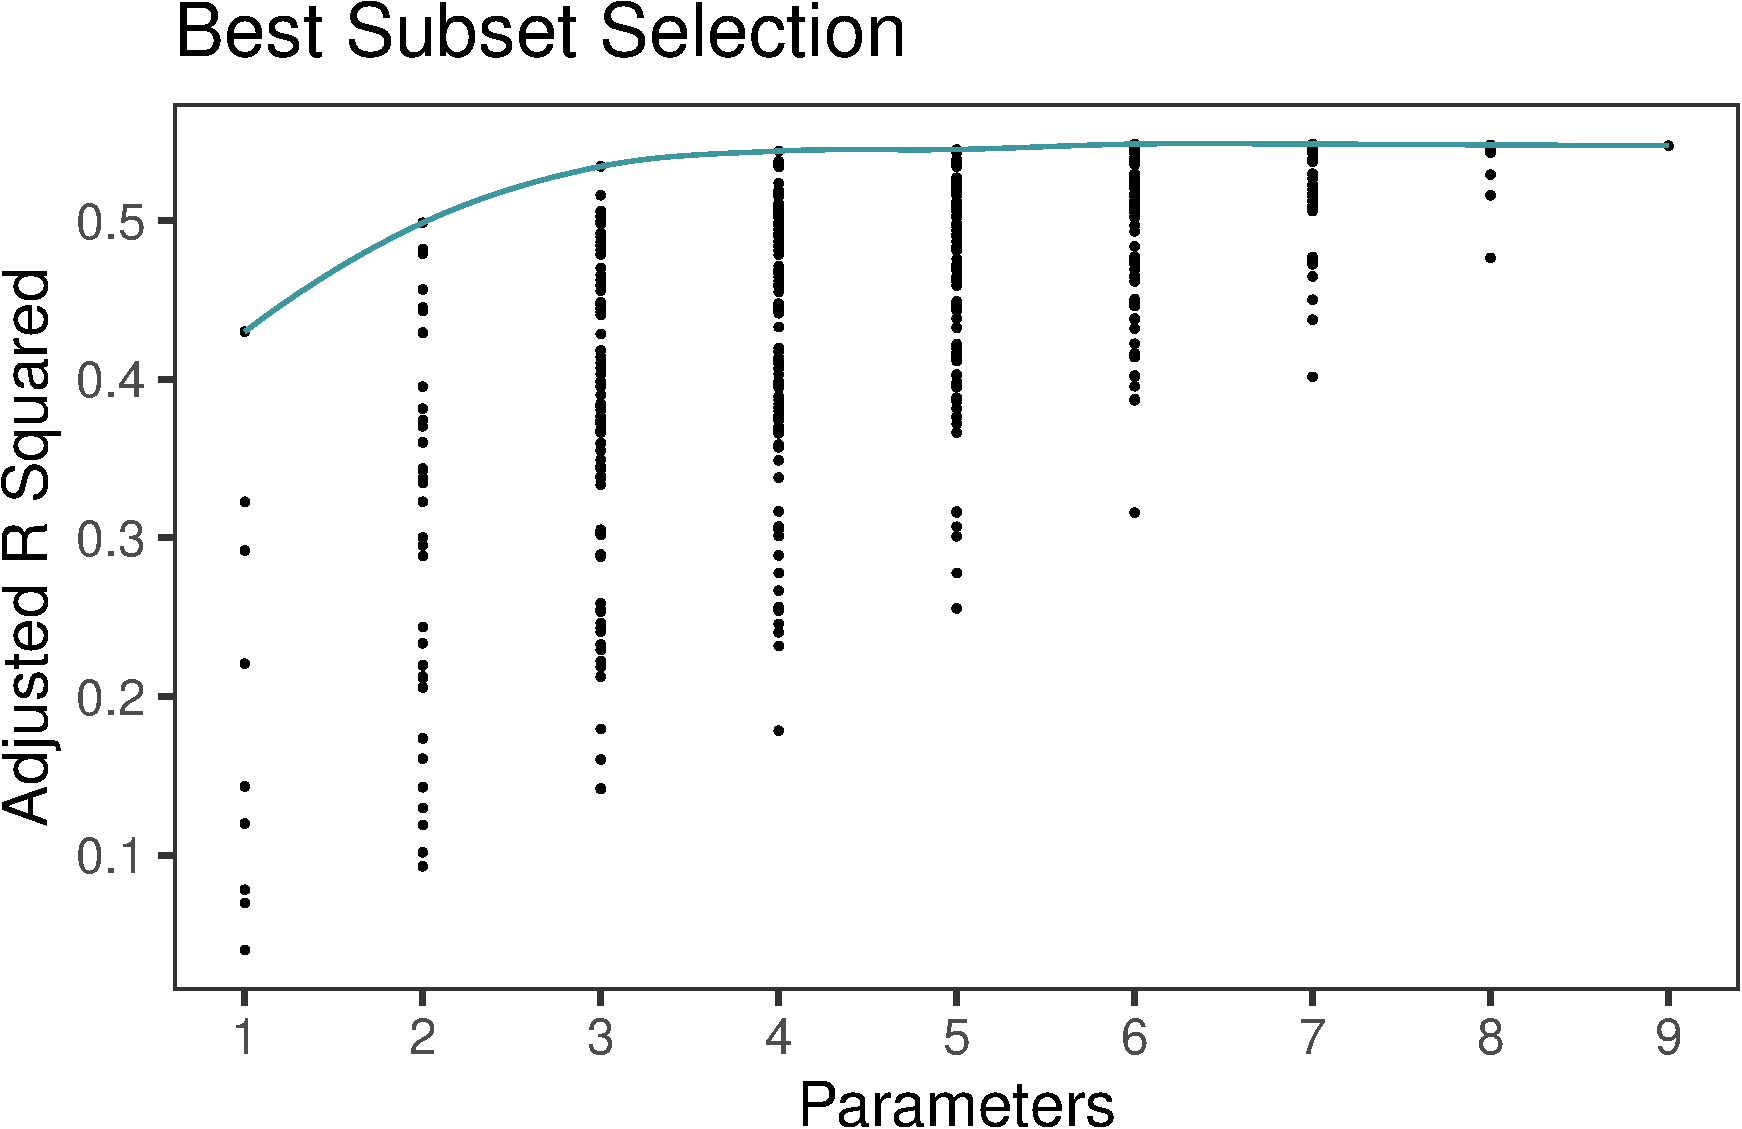
\includegraphics[width=0.5\linewidth]{paper_files/figure-latex/unnamed-chunk-3-1} 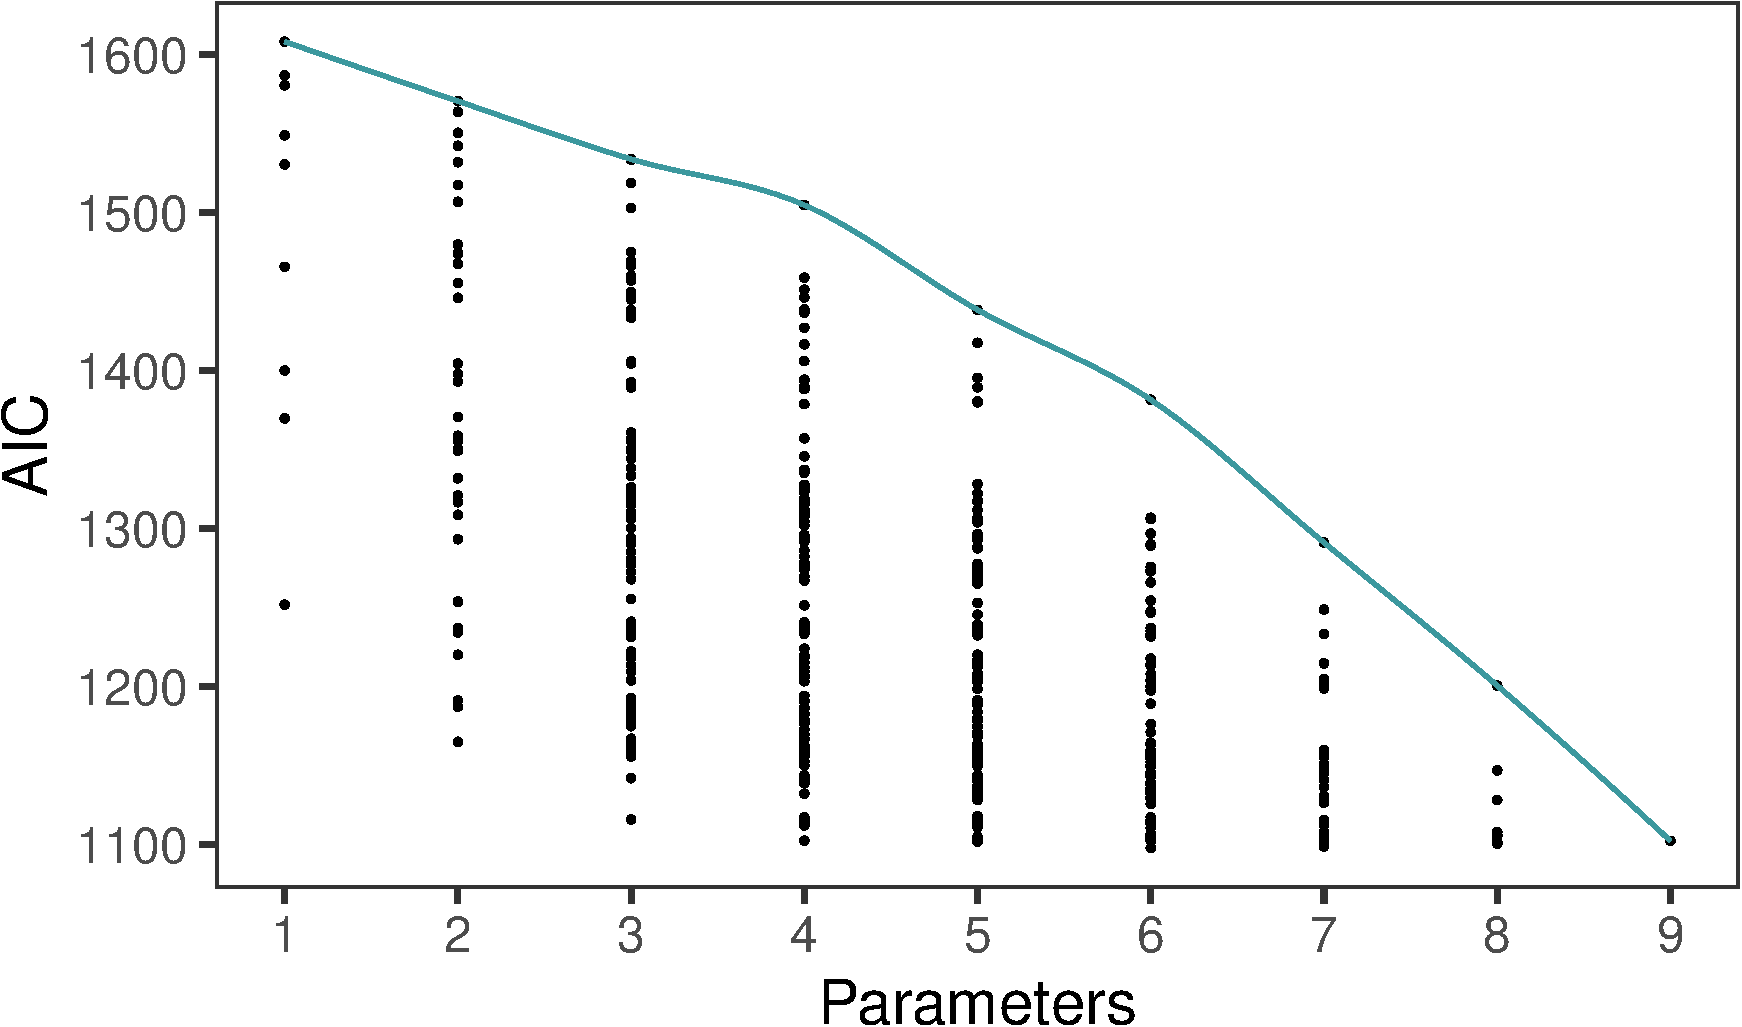
\includegraphics[width=0.5\linewidth]{paper_files/figure-latex/unnamed-chunk-3-2} \caption{ }\label{fig:unnamed-chunk-3}
\end{figure}

\hypertarget{model-selection}{%
\subsection{Model Selection}\label{model-selection}}

To select a model we performed the best subset algorithm to select several models with the best fit. Graphing the performance of each subset, we can see that the increase in \(R^{2}_a\) and \(AIC\) by adding additional parameters diminishes quite rapidly. It was appropriate to narrow our model choices down to three. First, the model with six degrees of freedom, one with five, and one with four. The results from these three models is in Table 2 made using the Stargazer package (Hlavac, 2018). The model with six degrees of freedom contains \textbf{Internet Users} with coefficient 0.003, which is statistically significant, however, a one percent increase in the percentage of people using the internet is associated with a 0.003 increase in political freedom is not politically significant. A coefficient that small has us suspecting that the relation that does not seem practically significant. Also, given the violation of assumptions it seems reasonable to exclude it from the model. Looking at the model with five degrees of freedom, all of our coefficients are significant at the 99\% level and seem large enough to be indicative of a linear association. The model with four degrees of freedom also has statistically significant coefficients and we would pick it had life expectancy not been significant. This is how we arrived at the model with five degrees of freedom.

\begin{table}[!htbp] \centering 
  \caption{Regression Results} 
  \label{} 
\begin{tabular}{@{\extracolsep{5pt}}lccc} 
\\[-1.8ex]\hline 
\hline \\[-1.8ex] 
 & \multicolumn{3}{c}{Political Rights Index} \\ 
\cline{2-4} 
 & DF = 6 & DF = 5 & DF = 4 \\ 
\hline \\[-1.8ex] 
 Corruption Perception & $-$0.022$^{***}$ & $-$0.023$^{***}$ & $-$0.023$^{***}$ \\ 
  & (0.002) & (0.002) & (0.002) \\ 
  Education Expendature & 1.655$^{***}$ & 2.076$^{***}$ & 2.064$^{***}$ \\ 
  & (0.550) & (0.525) & (0.526) \\ 
  Internet Users & 0.003$^{**}$ &  &  \\ 
  & (0.001) &  &  \\ 
  Life Expectancy & $-$0.024$^{***}$ & $-$0.013 &  \\ 
  & (0.009) & (0.008) &  \\ 
  Military Spending & $-$0.149$^{***}$ & $-$0.160$^{***}$ & $-$0.162$^{***}$ \\ 
  & (0.019) & (0.018) & (0.018) \\ 
  Murder Rate & $-$0.034$^{***}$ & $-$0.033$^{***}$ & $-$0.031$^{***}$ \\ 
  & (0.004) & (0.004) & (0.004) \\ 
  Intercept & 9.035$^{***}$ & 8.306$^{***}$ & 7.264$^{***}$ \\ 
  & (0.731) & (0.672) & (0.120) \\ 
 \hline \\[-1.8ex] 
Observations & 684 & 684 & 684 \\ 
R$^{2}$ & 0.552 & 0.548 & 0.546 \\ 
Adjusted R$^{2}$ & 0.548 & 0.545 & 0.544 \\ 
Residual Std. Error & 0.536 & 0.538 & 0.539 \\ 
F Statistic & 139.150$^{***}$ & 164.500$^{***}$ & 204.559$^{***}$ \\ 
\hline 
\hline \\[-1.8ex] 
Note: Standard Errors are in Prentices & \multicolumn{3}{r}{$^{*}$p$<$0.1; $^{**}$p$<$0.05; $^{***}$p$<$0.01} \\ 
\end{tabular} 
\end{table}

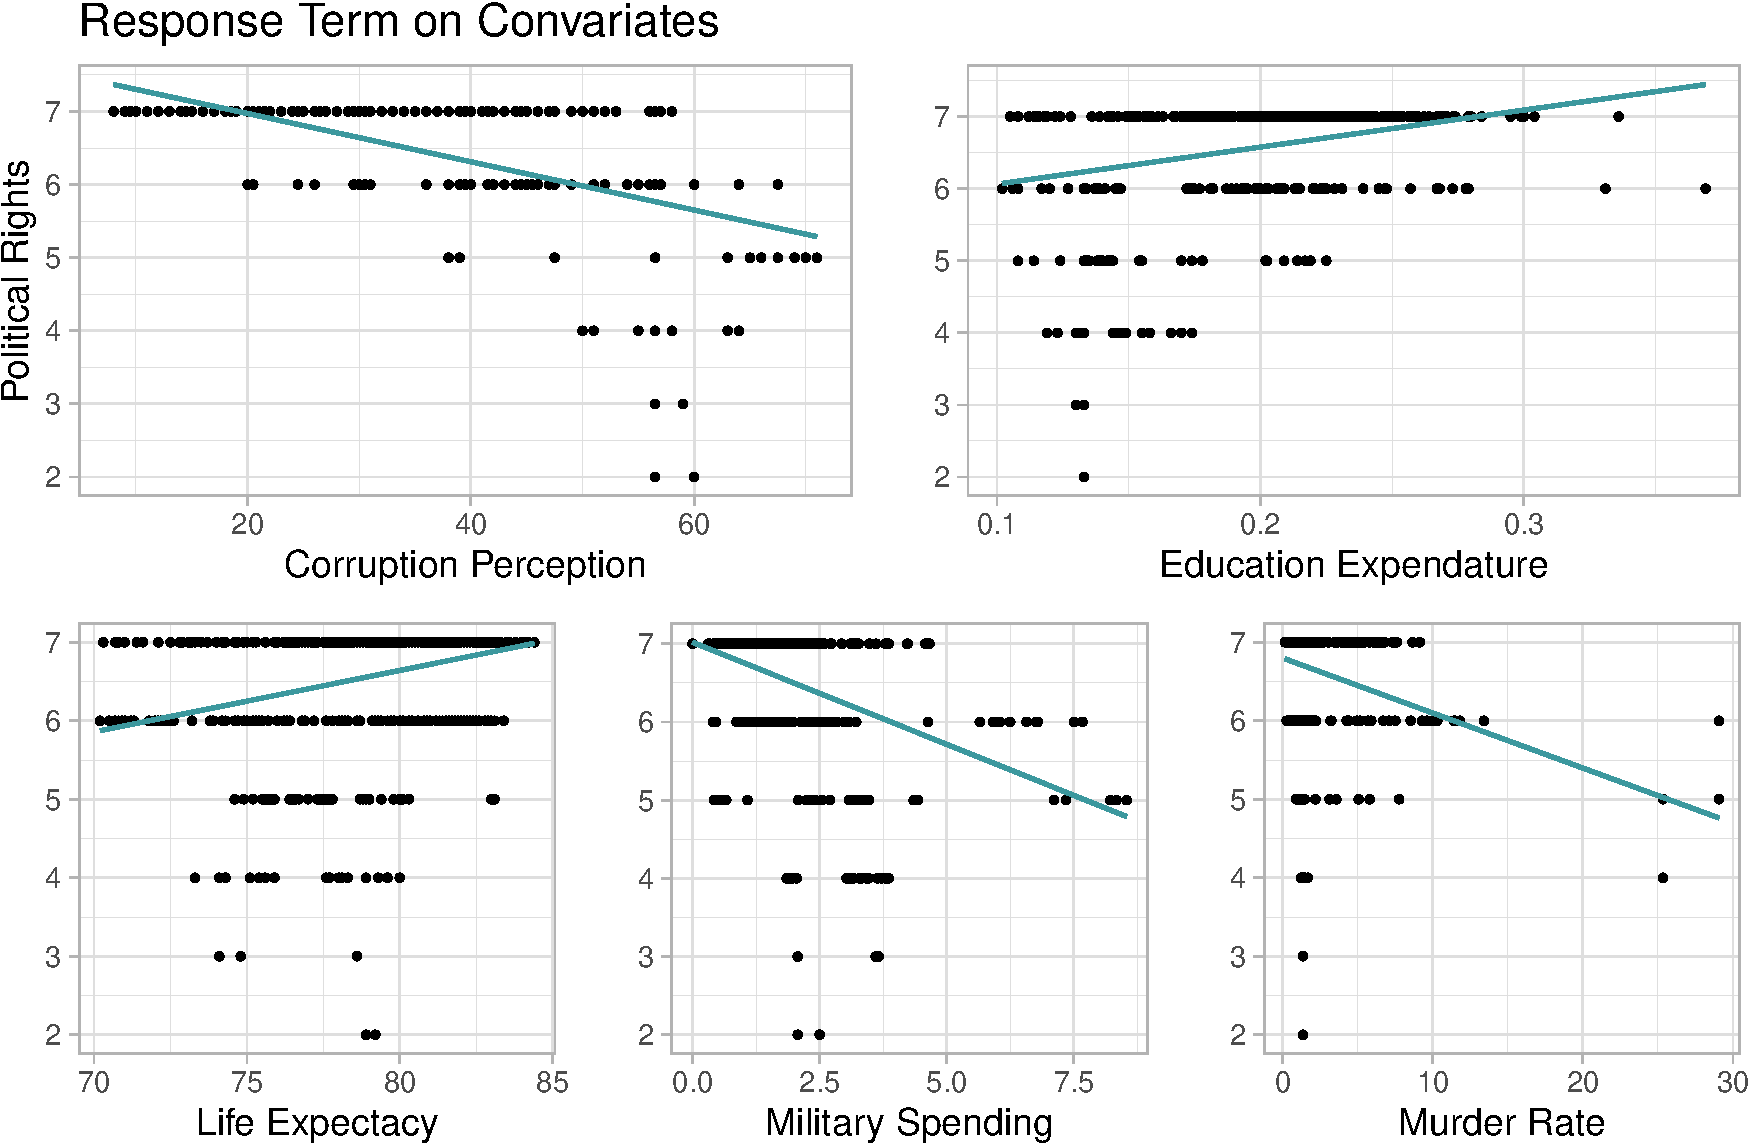
\includegraphics{paper_files/figure-latex/unnamed-chunk-5-1.pdf}

The scatter plots look a bit strange at first because of the nature of the discrete response variable, however, this does seem to fit the data reasonably well. There is a fairly linear relationship with a clear sloping line which, except for life expectancy, concur with the regression coefficients. Life expectancy on it's own has a positive association with political freedom, however, when holding the other covariates constant we find that association to be negative.

Now we will examine some regression diagnostics to analyze the performance and identify problems. Let's start with plots of residuals. Figure 2, contains a histogram of the residuals adjacent to a QQ normal plot. It is clear that there are substantial outliers at the lower end of political freedom. Upon further inspection, we found that these outliers are Turkey from 2016 to 2018. These residuals are large and suggest a substantial loss in political freedom. This is confirmed by Freedomhouse (\emph{Countries and territories}, 2020) reporting that a coup attempt in Turkey resulted in a political retaliation against perceived opponents and constitutional changes were made that concentrated political power to the president. After some discussion, we concluded that since the regression results were not severely affected and this is not an entry error removing these data points is inappropriate.

It was clear from the plots that error variance may not be constant. A Brown-Forsythe test confirmed our suspicions informing us that the error variance is not consistent. We calculated a \(t^{*}_{BF} = 9.49\) indicating the error variance is substantially higher when the values of political freedom are lower. This is likely due to the fact that our sample includes predominately values that are on the upper end of the political freedom.

\begin{figure}
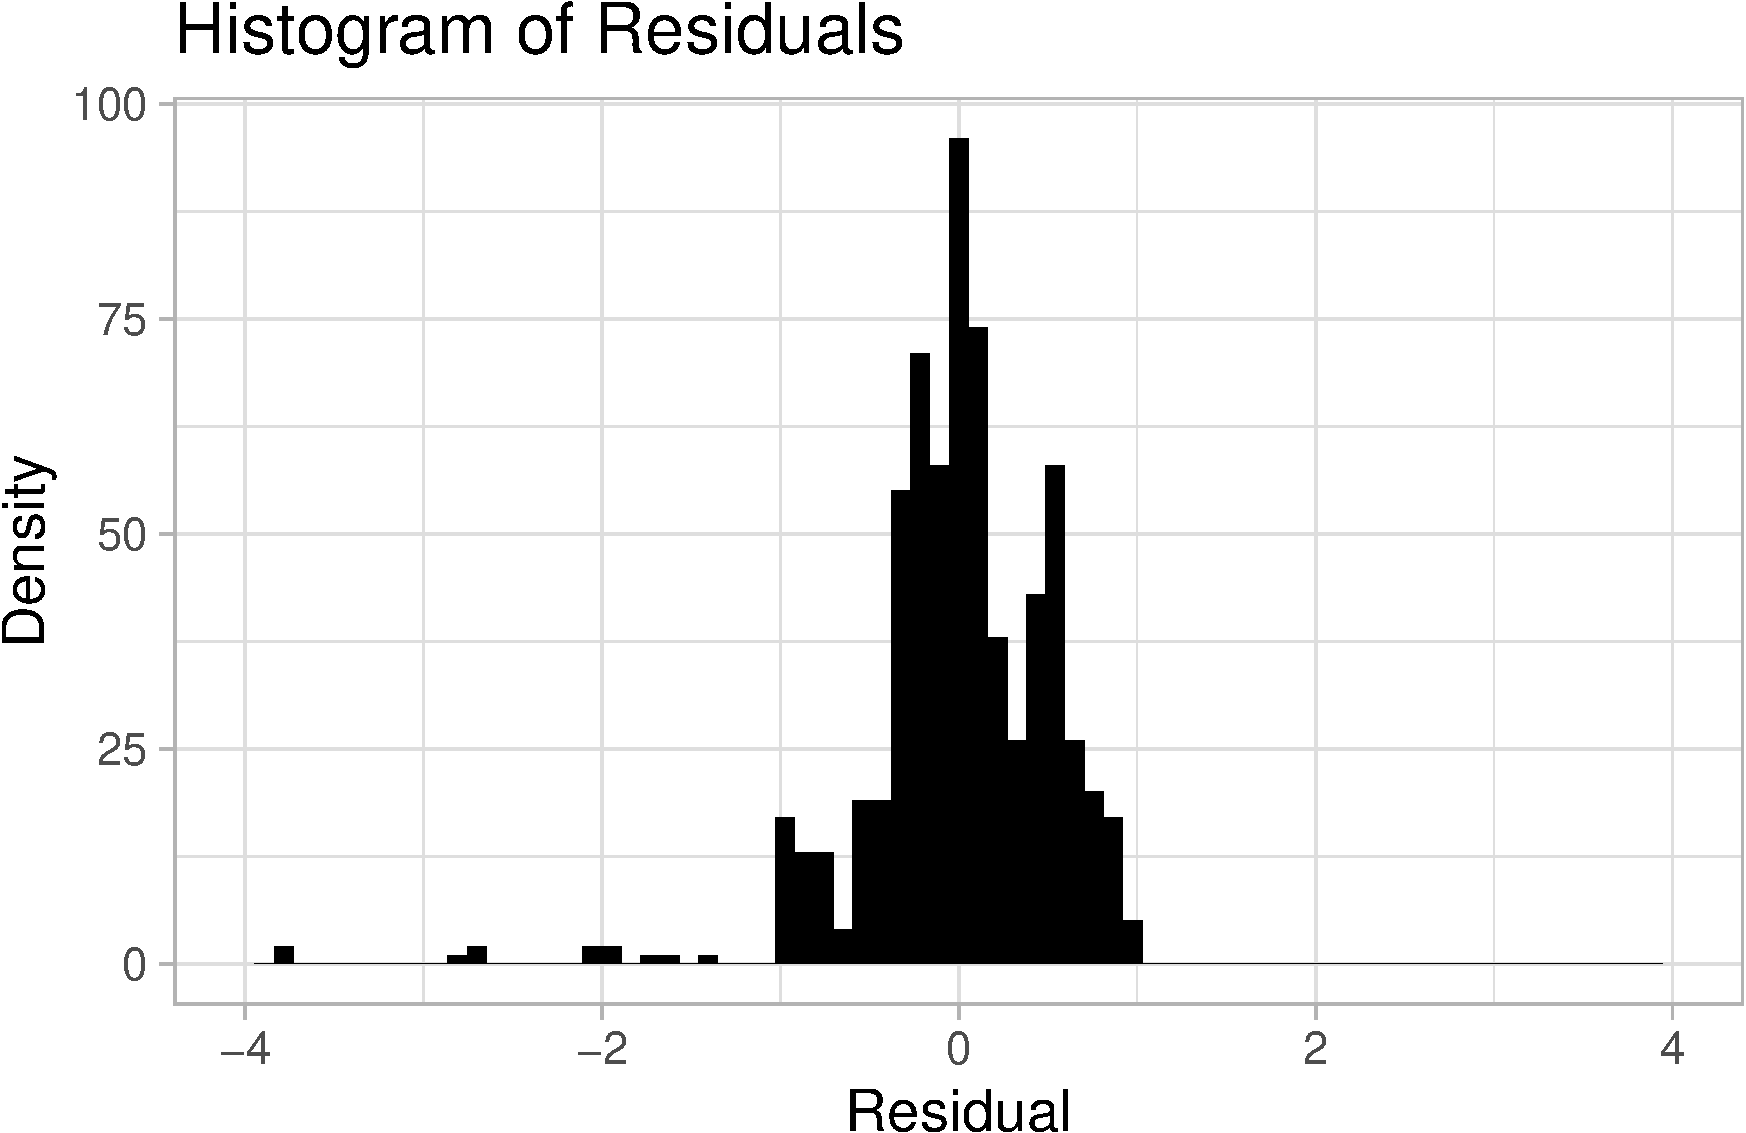
\includegraphics[width=0.5\linewidth]{paper_files/figure-latex/unnamed-chunk-6-1} 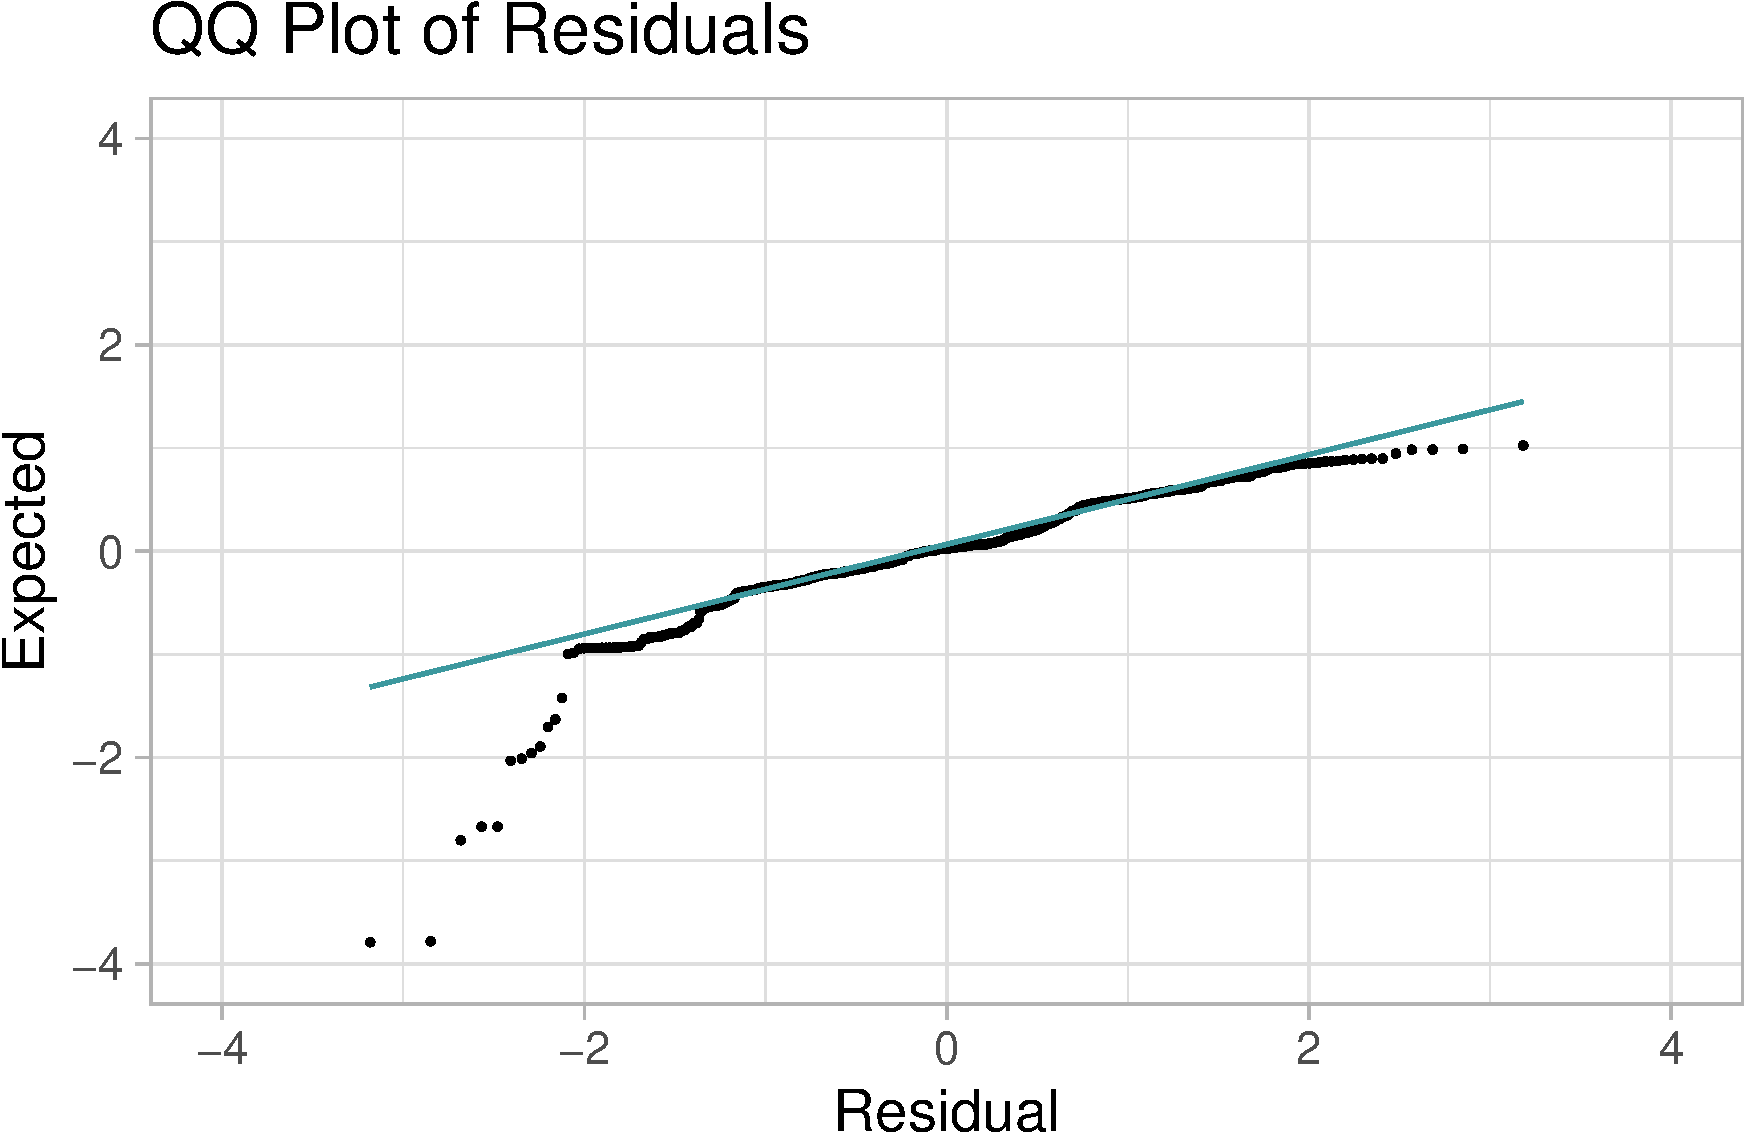
\includegraphics[width=0.5\linewidth]{paper_files/figure-latex/unnamed-chunk-6-2} \caption{ }\label{fig:unnamed-chunk-6}
\end{figure}

\hypertarget{conclusion}{%
\subsection{Conclusion}\label{conclusion}}

The results are statistically significant but can only be interpreted for countries in the OECD. The model performs reasonably well explaining the political freedom of countries in the 6 and 7 range. However, the model completely falls apart at the one case of a substantial loss in freedom. Again, we don't have an exhaustive sample of countries losing freedom so this is consistent with the dataset we have. However, we can conclude as one of our more robust results is that an increase in education expenditure is associated with an increase in political freedom. The less corrupt a country is perceived to be the more freedom the citizens are afforded. Military spending is associated with a decrease in political freedom.
After conducting this study, we are reasonably sure that a relationship exists between political freedom and social, economic, and political factors. We are assured these things matter. Therefore, because we value political freedom, we suggest that when the choice comes, policy makers should choose to spend on education opposed to military when attempting to increase political freedom. Other covariates, policy makers do not have such direct control over.

\newpage

\hypertarget{references}{%
\section{References}\label{references}}

\begingroup
\setlength{\parindent}{-0.5in}
\setlength{\leftskip}{0.5in}

\hypertarget{refs}{}
\begin{CSLReferences}{1}{0}
\leavevmode\hypertarget{ref-R-papaja}{}%
Aust, F., \& Barth, M. (2020). \emph{{papaja}: {Create} {APA} manuscripts with {R Markdown}}. Retrieved from \url{https://github.com/crsh/papaja}

\leavevmode\hypertarget{ref-Freedomhouse}{}%
\emph{Countries and territories}. (2020). Washington D.C.: Freedomhouse. Retrieved from \url{https://freedomhouse.org}

\leavevmode\hypertarget{ref-R-stargazer}{}%
Hlavac, M. (2018). \emph{Stargazer: Well-formatted regression and summary statistics tables}. Bratislava, Slovakia: Central European Labour Studies Institute (CELSI). Retrieved from \url{https://CRAN.R-project.org/package=stargazer}

\leavevmode\hypertarget{ref-R-base}{}%
R Core Team. (2020). \emph{R: A language and environment for statistical computing}. Vienna, Austria: R Foundation for Statistical Computing. Retrieved from \url{https://www.R-project.org/}

\leavevmode\hypertarget{ref-Gapminder}{}%
Rosling, H. (2020). \emph{Gapminder}. Retrieved from \url{https://www.gapminder.org/data/}

\leavevmode\hypertarget{ref-R-tidyverse}{}%
Wickham, H., Averick, M., Bryan, J., Chang, W., McGowan, L. D., François, R., \ldots{} Yutani, H. (2019). Welcome to the {tidyverse}. \emph{Journal of Open Source Software}, \emph{4}(43), 1686. \url{https://doi.org/10.21105/joss.01686}

\leavevmode\hypertarget{ref-R-kableExtra}{}%
Zhu, H. (2020). \emph{kableExtra: Construct complex table with 'kable' and pipe syntax}. Retrieved from \url{https://CRAN.R-project.org/package=kableExtra}

\end{CSLReferences}

\endgroup

\newpage

\hypertarget{appendix-all-code-for-this-report}{%
\section{Appendix: All code for this report}\label{appendix-all-code-for-this-report}}

\begin{Shaded}
\begin{Highlighting}[]
\FunctionTok{library}\NormalTok{(tidyverse)}
\FunctionTok{library}\NormalTok{(kableExtra)}
\FunctionTok{library}\NormalTok{(stargazer)}
\FunctionTok{library}\NormalTok{(patchwork)}
\FunctionTok{library}\NormalTok{(}\StringTok{"papaja"}\NormalTok{)}
\NormalTok{size }\OtherTok{\textless{}{-}} \DecValTok{30}
\FunctionTok{r\_refs}\NormalTok{(}\StringTok{"r{-}references.bib"}\NormalTok{)}
\NormalTok{knitr}\SpecialCharTok{::}\NormalTok{opts\_chunk}\SpecialCharTok{$}\FunctionTok{set}\NormalTok{(}\AttributeTok{echo =} \ConstantTok{FALSE}\NormalTok{, }\AttributeTok{warning=}\ConstantTok{FALSE}\NormalTok{, }\AttributeTok{message =} \ConstantTok{FALSE}\NormalTok{, }
                      \AttributeTok{fig.width =} \DecValTok{12}\NormalTok{, }\AttributeTok{fig.height =} \DecValTok{8}\NormalTok{) }
\CommentTok{\# Read and Clean {-}{-}{-}{-}{-}{-}{-}{-}{-}{-}{-}{-}{-}{-}{-}{-}{-}{-}{-}{-}{-}{-}{-}{-}{-}{-}{-}{-}{-}{-}{-}{-}{-}{-}{-}{-}{-}{-}{-}{-}{-}{-}{-}{-}{-}{-}{-}{-}{-}{-}{-}{-}{-}{-}{-}{-}{-}{-}}
\NormalTok{files }\OtherTok{\textless{}{-}} \FunctionTok{list.files}\NormalTok{(}\AttributeTok{path =}\NormalTok{ here}\SpecialCharTok{::}\FunctionTok{here}\NormalTok{(}\StringTok{"raw\_data"}\NormalTok{), }\AttributeTok{pattern =} \StringTok{".csv"}\NormalTok{)}
\NormalTok{cleaning }\OtherTok{\textless{}{-}} \ControlFlowTok{function}\NormalTok{(df)\{}
\NormalTok{  df }\OtherTok{\textless{}{-}} \FunctionTok{pivot\_longer}\NormalTok{(df, }\AttributeTok{cols =} \SpecialCharTok{{-}}\NormalTok{country, }\AttributeTok{names\_to =} \StringTok{"year"}\NormalTok{)}
\NormalTok{\}}
\NormalTok{data }\OtherTok{\textless{}{-}}\NormalTok{ files }\SpecialCharTok{\%\textgreater{}\%} 
  \FunctionTok{map}\NormalTok{(}\ControlFlowTok{function}\NormalTok{(x) }\FunctionTok{read\_csv}\NormalTok{(}\FunctionTok{paste0}\NormalTok{(}\StringTok{"raw\_data/"}\NormalTok{, x))) }\SpecialCharTok{\%\textgreater{}\%} 
  \FunctionTok{setNames}\NormalTok{(}\FunctionTok{gsub}\NormalTok{(}\StringTok{"}\SpecialCharTok{\textbackslash{}\textbackslash{}}\StringTok{.csv$"}\NormalTok{, }\StringTok{""}\NormalTok{, files)) }\SpecialCharTok{\%\textgreater{}\%} 
  \FunctionTok{map}\NormalTok{(cleaning) }\SpecialCharTok{\%\textgreater{}\%} 
  \FunctionTok{bind\_rows}\NormalTok{(}\AttributeTok{.id =} \StringTok{"id"}\NormalTok{) }\SpecialCharTok{\%\textgreater{}\%} 
  \FunctionTok{pivot\_wider}\NormalTok{(}\AttributeTok{names\_from =}\NormalTok{ id)}
\CommentTok{\# Filtering {-}{-}{-}{-}{-}{-}{-}{-}{-}{-}{-}{-}{-}{-}{-}{-}{-}{-}{-}{-}{-}{-}{-}{-}{-}{-}{-}{-}{-}{-}{-}{-}{-}{-}{-}{-}{-}{-}{-}{-}{-}{-}{-}{-}{-}{-}{-}{-}{-}{-}{-}{-}{-}{-}{-}{-}{-}{-}{-}{-}{-}{-}{-}}
\NormalTok{countries }\OtherTok{\textless{}{-}} \FunctionTok{readRDS}\NormalTok{(here}\SpecialCharTok{::}\FunctionTok{here}\NormalTok{(}\StringTok{"data"}\NormalTok{, }\StringTok{"countries.RDS"}\NormalTok{))}
\NormalTok{data }\OtherTok{\textless{}{-}}\NormalTok{ data }\SpecialCharTok{\%\textgreater{}\%}
  \FunctionTok{mutate}\NormalTok{(}\AttributeTok{year =} \FunctionTok{as.numeric}\NormalTok{(year)) }\SpecialCharTok{\%\textgreater{}\%} 
  \FunctionTok{filter}\NormalTok{(year }\SpecialCharTok{\textgreater{}=} \DecValTok{2000}\NormalTok{, year }\SpecialCharTok{\textless{}} \DecValTok{2019}\NormalTok{, country }\SpecialCharTok{\%in\%}\NormalTok{ countries) }\SpecialCharTok{\%\textgreater{}\%} 
  \FunctionTok{group\_by}\NormalTok{(country) }\SpecialCharTok{\%\textgreater{}\%}
  \FunctionTok{mutate\_at}\NormalTok{(}\FunctionTok{vars}\NormalTok{(}\SpecialCharTok{{-}}\NormalTok{country),}\FunctionTok{list}\NormalTok{(}\SpecialCharTok{\textasciitilde{}}\FunctionTok{ifelse}\NormalTok{(}\FunctionTok{is.na}\NormalTok{(.), }\FunctionTok{median}\NormalTok{(., }\AttributeTok{na.rm =} \ConstantTok{TRUE}\NormalTok{), .))) }\SpecialCharTok{\%\textgreater{}\%} 
\CommentTok{\# Iceland spent 0 so I needed to manually recode that}
  \FunctionTok{mutate}\NormalTok{(}\AttributeTok{military\_spending\_pct\_of\_gdp =} \FunctionTok{replace\_na}\NormalTok{(military\_spending\_pct\_of\_gdp, }\DecValTok{0}\NormalTok{),}
         \AttributeTok{murder\_per\_mil\_people =} \FunctionTok{replace}\NormalTok{(murder\_per\_mil\_people, country }\SpecialCharTok{==} \StringTok{"Mexico"}\NormalTok{, }\FloatTok{29.07}\NormalTok{),}
         \AttributeTok{murder\_per\_mil\_people =} \FunctionTok{replace}\NormalTok{(murder\_per\_mil\_people, country }\SpecialCharTok{==} \StringTok{"Chile"}\NormalTok{, }\FloatTok{4.4}\NormalTok{),}
         \AttributeTok{murder\_per\_mil\_people =} \FunctionTok{replace}\NormalTok{(murder\_per\_mil\_people, country }\SpecialCharTok{==} \StringTok{"Colombia"}\NormalTok{, }\FloatTok{25.34}\NormalTok{)) }\SpecialCharTok{\%\textgreater{}\%} 
  \FunctionTok{relocate}\NormalTok{(polrights\_fh) }\SpecialCharTok{\%\textgreater{}\%} 
  \FunctionTok{mutate}\NormalTok{(}\AttributeTok{polrights\_fh =}\NormalTok{ (}\DecValTok{8} \SpecialCharTok{{-}}\NormalTok{ polrights\_fh),}
 \AttributeTok{military\_spending\_pct\_of\_gdp =}\NormalTok{ military\_spending\_pct\_of\_gdp }\SpecialCharTok{*} \DecValTok{100}\NormalTok{) }\SpecialCharTok{\%\textgreater{}\%} 
  \FunctionTok{mutate}\NormalTok{(}\AttributeTok{corruption\_perception\_index\_cpi =}\NormalTok{ (}\DecValTok{100} \SpecialCharTok{{-}}\NormalTok{ corruption\_perception\_index\_cpi)) }\SpecialCharTok{\%\textgreater{}\%} 
  \FunctionTok{ungroup}\NormalTok{()}
\CommentTok{\# Best Subset Selection {-}{-}{-}{-}{-}{-}{-}{-}{-}{-}{-}{-}{-}{-}{-}{-}{-}{-}{-}{-}{-}{-}{-}{-}{-}{-}{-}{-}{-}{-}{-}{-}{-}{-}{-}{-}{-}{-}{-}{-}{-}{-}{-}{-}{-}{-}{-}{-}{-}{-}{-}{-}{-}{-}{-}{-}{-}{-}{-}{-}{-}{-}{-}}
\NormalTok{vars }\OtherTok{\textless{}{-}}\NormalTok{ data }\SpecialCharTok{\%\textgreater{}\%} 
  \FunctionTok{select}\NormalTok{(}\SpecialCharTok{{-}}\NormalTok{country, }\SpecialCharTok{{-}}\NormalTok{year, }\SpecialCharTok{{-}}\FunctionTok{ends\_with}\NormalTok{(}\StringTok{"\_fh"}\NormalTok{)) }\SpecialCharTok{\%\textgreater{}\%}
  \FunctionTok{names}\NormalTok{()}
\NormalTok{models }\OtherTok{\textless{}{-}} \FunctionTok{list}\NormalTok{()}
\ControlFlowTok{for}\NormalTok{ (i }\ControlFlowTok{in} \DecValTok{1}\SpecialCharTok{:}\FunctionTok{length}\NormalTok{(vars)) \{}
\NormalTok{  vc }\OtherTok{\textless{}{-}} \FunctionTok{combn}\NormalTok{(vars,i)}
  \ControlFlowTok{for}\NormalTok{ (j }\ControlFlowTok{in} \DecValTok{1}\SpecialCharTok{:}\FunctionTok{ncol}\NormalTok{(vc)) \{}
\NormalTok{    model }\OtherTok{\textless{}{-}} \FunctionTok{as.formula}\NormalTok{(}\FunctionTok{paste0}\NormalTok{(}\StringTok{"polrights\_fh"}\NormalTok{, }\StringTok{" \textasciitilde{}"}\NormalTok{, }\FunctionTok{paste0}\NormalTok{(vc[,j], }\AttributeTok{collapse =} \StringTok{" + "}\NormalTok{)))}
\NormalTok{    models }\OtherTok{\textless{}{-}} \FunctionTok{c}\NormalTok{(models, model)}
\NormalTok{    \}}
\NormalTok{  \}}
\NormalTok{subsets }\OtherTok{\textless{}{-}} \FunctionTok{map}\NormalTok{(models, }\ControlFlowTok{function}\NormalTok{(x) }\FunctionTok{lm}\NormalTok{(x, data)) }\SpecialCharTok{\%\textgreater{}\%} 
  \FunctionTok{map}\NormalTok{(broom}\SpecialCharTok{::}\NormalTok{glance) }\SpecialCharTok{\%\textgreater{}\%} 
  \FunctionTok{setNames}\NormalTok{(models) }\SpecialCharTok{\%\textgreater{}\%} 
  \FunctionTok{bind\_rows}\NormalTok{(}\AttributeTok{.id =} \StringTok{"id"}\NormalTok{) }\SpecialCharTok{\%\textgreater{}\%} 
  \FunctionTok{rename}\NormalTok{(}\AttributeTok{model =}\NormalTok{ id) }\SpecialCharTok{\%\textgreater{}\%} 
  \FunctionTok{mutate}\NormalTok{(}\AttributeTok{Model =} \FunctionTok{str\_replace\_all}\NormalTok{(model, }\StringTok{"\_"}\NormalTok{, }\StringTok{" "}\NormalTok{),}
         \AttributeTok{Model =} \FunctionTok{str\_replace}\NormalTok{(Model, }\StringTok{"\textasciitilde{}"}\NormalTok{, }\StringTok{"="}\NormalTok{), }
         \AttributeTok{Model =} \FunctionTok{str\_to\_title}\NormalTok{(Model))}
\NormalTok{model\_df6\_formula }\OtherTok{\textless{}{-}}\NormalTok{ subsets }\SpecialCharTok{\%\textgreater{}\%} \FunctionTok{filter}\NormalTok{(df }\SpecialCharTok{==} \DecValTok{6}\NormalTok{) }\SpecialCharTok{\%\textgreater{}\%} 
  \FunctionTok{arrange}\NormalTok{(}\FunctionTok{desc}\NormalTok{(adj.r.squared)) }\SpecialCharTok{\%\textgreater{}\%} 
  \FunctionTok{select}\NormalTok{(model) }\SpecialCharTok{\%\textgreater{}\%} \FunctionTok{head}\NormalTok{(}\DecValTok{1}\NormalTok{) }\SpecialCharTok{\%\textgreater{}\%} \FunctionTok{as.character}\NormalTok{() }
\NormalTok{fit\_df6 }\OtherTok{\textless{}{-}} \FunctionTok{lm}\NormalTok{(model\_df6\_formula, data)}
\NormalTok{model\_df5\_formula }\OtherTok{\textless{}{-}}\NormalTok{ subsets }\SpecialCharTok{\%\textgreater{}\%} \FunctionTok{filter}\NormalTok{(df }\SpecialCharTok{==} \DecValTok{5}\NormalTok{) }\SpecialCharTok{\%\textgreater{}\%} 
  \FunctionTok{arrange}\NormalTok{(}\FunctionTok{desc}\NormalTok{(adj.r.squared)) }\SpecialCharTok{\%\textgreater{}\%} 
  \FunctionTok{select}\NormalTok{(model) }\SpecialCharTok{\%\textgreater{}\%} \FunctionTok{head}\NormalTok{(}\DecValTok{1}\NormalTok{) }\SpecialCharTok{\%\textgreater{}\%} \FunctionTok{as.character}\NormalTok{()}
\NormalTok{fit\_df5 }\OtherTok{\textless{}{-}} \FunctionTok{lm}\NormalTok{(model\_df5\_formula, data)}
\NormalTok{model\_df4\_formula }\OtherTok{\textless{}{-}}\NormalTok{ subsets }\SpecialCharTok{\%\textgreater{}\%} \FunctionTok{filter}\NormalTok{(df }\SpecialCharTok{==} \DecValTok{4}\NormalTok{) }\SpecialCharTok{\%\textgreater{}\%} 
  \FunctionTok{arrange}\NormalTok{(}\FunctionTok{desc}\NormalTok{(adj.r.squared)) }\SpecialCharTok{\%\textgreater{}\%} 
  \FunctionTok{select}\NormalTok{(model) }\SpecialCharTok{\%\textgreater{}\%} \FunctionTok{head}\NormalTok{(}\DecValTok{1}\NormalTok{) }\SpecialCharTok{\%\textgreater{}\%} \FunctionTok{as.character}\NormalTok{() }
\NormalTok{fit\_df4 }\OtherTok{\textless{}{-}} \FunctionTok{lm}\NormalTok{(model\_df4\_formula, data)}
\NormalTok{stat }\OtherTok{\textless{}{-}} \ControlFlowTok{function}\NormalTok{(x, }\AttributeTok{df =}\NormalTok{ data, }\AttributeTok{rounding\_digits =} \DecValTok{2}\NormalTok{)\{}
\NormalTok{    x }\OtherTok{\textless{}{-}} \FunctionTok{enquo}\NormalTok{(x)}
\NormalTok{    df }\SpecialCharTok{\%\textgreater{}\%}
      \FunctionTok{summarise}\NormalTok{(}
                       \AttributeTok{Mean  =} \FunctionTok{mean}\NormalTok{( }\SpecialCharTok{!!}\NormalTok{ x),}
                     \AttributeTok{Median  =} \FunctionTok{median}\NormalTok{( }\SpecialCharTok{!!}\NormalTok{ x),}
                         \AttributeTok{Std =} \FunctionTok{sd}\NormalTok{  ( }\SpecialCharTok{!!}\NormalTok{ x),}
                         \AttributeTok{Min =} \FunctionTok{min}\NormalTok{ ( }\SpecialCharTok{!!}\NormalTok{ x),}
                         \AttributeTok{Max =} \FunctionTok{max}\NormalTok{ ( }\SpecialCharTok{!!}\NormalTok{ x),}
                       \AttributeTok{Range =} \FunctionTok{max}\NormalTok{(}\SpecialCharTok{!!}\NormalTok{ x) }\SpecialCharTok{{-}} \FunctionTok{min}\NormalTok{(}\SpecialCharTok{!!}\NormalTok{ x) ) }\SpecialCharTok{\%\textgreater{}\%}
      \FunctionTok{mutate\_if}\NormalTok{(is.numeric, round, rounding\_digits)}
\NormalTok{\}}
\NormalTok{data }\SpecialCharTok{\%\textgreater{}\%} 
  \FunctionTok{select}\NormalTok{(}\SpecialCharTok{{-}}\NormalTok{country) }\SpecialCharTok{\%\textgreater{}\%} 
\FunctionTok{map}\NormalTok{(}\ControlFlowTok{function}\NormalTok{(x)\{}\FunctionTok{stat}\NormalTok{(x)\}) }\SpecialCharTok{\%\textgreater{}\%} 
  \FunctionTok{bind\_rows}\NormalTok{(}\AttributeTok{.id =} \StringTok{"Variable"}\NormalTok{) }\SpecialCharTok{\%\textgreater{}\%} 
  \FunctionTok{mutate}\NormalTok{(}\AttributeTok{Variable =} \FunctionTok{replace}\NormalTok{(Variable, }
                            \AttributeTok{values =} \FunctionTok{c}\NormalTok{(}\StringTok{"Political Rights"}\NormalTok{, }\StringTok{"Year"}\NormalTok{, }
                                       \StringTok{"Corruption Perception"}\NormalTok{, }
                                       \StringTok{"Education Expenditure"}\NormalTok{, }
                                       \StringTok{"Electricity Use"}\NormalTok{, }
                                       \StringTok{"Gini"}\NormalTok{, }
                                       \StringTok{"Internet Users"}\NormalTok{,}
                                       \StringTok{"Life Expectancy"}\NormalTok{, }
                                       \StringTok{"Labor Force Participation"}\NormalTok{, }
                                       \StringTok{"Military Spending"}\NormalTok{, }
                                       \StringTok{"Murders rate"}\NormalTok{))) }\SpecialCharTok{\%\textgreater{}\%} 
\FunctionTok{kable}\NormalTok{(}
  \AttributeTok{format =} \StringTok{"latex"}\NormalTok{,}
  \AttributeTok{booktabs =} \ConstantTok{TRUE}\NormalTok{,}
  \AttributeTok{escape =} \ConstantTok{FALSE}\NormalTok{,}
  \AttributeTok{longtable =} \ConstantTok{TRUE}\NormalTok{,}
 \AttributeTok{caption =} \StringTok{"Descriptive Statistics"}\NormalTok{)}
\NormalTok{r }\OtherTok{\textless{}{-}}\NormalTok{ subsets }\SpecialCharTok{\%\textgreater{}\%} 
  \FunctionTok{group\_by}\NormalTok{(df) }\SpecialCharTok{\%\textgreater{}\%} 
  \FunctionTok{summarise}\NormalTok{(}\AttributeTok{adj =} \FunctionTok{max}\NormalTok{(adj.r.squared, }\AttributeTok{na.rm =}\NormalTok{ T))}

\NormalTok{subsets }\SpecialCharTok{\%\textgreater{}\%} 
  \FunctionTok{ggplot}\NormalTok{(}\FunctionTok{aes}\NormalTok{(}\AttributeTok{x =}\NormalTok{ df, }\AttributeTok{y =}\NormalTok{ adj.r.squared)) }\SpecialCharTok{+} 
  \FunctionTok{geom\_point}\NormalTok{() }\SpecialCharTok{+} 
  \FunctionTok{geom\_smooth}\NormalTok{(}\AttributeTok{data =}\NormalTok{ r, }\FunctionTok{aes}\NormalTok{(df, adj), }
              \AttributeTok{se =} \ConstantTok{FALSE}\NormalTok{, }\AttributeTok{span =} \FloatTok{0.5}\NormalTok{, }\AttributeTok{color =} \StringTok{"\#3C989E"}\NormalTok{) }\SpecialCharTok{+} 
  \FunctionTok{labs}\NormalTok{(}\AttributeTok{title =} \StringTok{""}\NormalTok{, }\AttributeTok{x =} \StringTok{"Parameters"}\NormalTok{, }\AttributeTok{y =} \StringTok{"Adjusted R Squared"}\NormalTok{) }\SpecialCharTok{+} 
  \FunctionTok{scale\_x\_continuous}\NormalTok{(}\AttributeTok{breaks =} \DecValTok{1}\SpecialCharTok{:}\DecValTok{9}\NormalTok{) }\SpecialCharTok{+} 
  \FunctionTok{theme\_test}\NormalTok{(}\AttributeTok{base\_size =}\NormalTok{ size) }\SpecialCharTok{+} \FunctionTok{labs}\NormalTok{(}\AttributeTok{title =} \StringTok{"Best Subset Selection"}\NormalTok{)}

\NormalTok{r }\OtherTok{\textless{}{-}}\NormalTok{ subsets }\SpecialCharTok{\%\textgreater{}\%} 
  \FunctionTok{group\_by}\NormalTok{(df) }\SpecialCharTok{\%\textgreater{}\%} 
  \FunctionTok{summarise}\NormalTok{(}\AttributeTok{AIC =} \FunctionTok{max}\NormalTok{(AIC, }\AttributeTok{na.rm =}\NormalTok{ T))}

\NormalTok{subsets }\SpecialCharTok{\%\textgreater{}\%} 
  \FunctionTok{ggplot}\NormalTok{(}\FunctionTok{aes}\NormalTok{(}\AttributeTok{x =}\NormalTok{ df, }\AttributeTok{y =}\NormalTok{ AIC)) }\SpecialCharTok{+} 
  \FunctionTok{geom\_point}\NormalTok{() }\SpecialCharTok{+} 
  \FunctionTok{geom\_smooth}\NormalTok{(}\AttributeTok{data =}\NormalTok{ r, }\FunctionTok{aes}\NormalTok{(df, AIC), }
              \AttributeTok{se =} \ConstantTok{FALSE}\NormalTok{, }\AttributeTok{span =} \FloatTok{0.5}\NormalTok{, }\AttributeTok{color =} \StringTok{"\#3C989E"}\NormalTok{) }\SpecialCharTok{+} 
  \FunctionTok{labs}\NormalTok{(}\AttributeTok{title =} \StringTok{""}\NormalTok{, }\AttributeTok{x =} \StringTok{"Parameters"}\NormalTok{, }\AttributeTok{y =} \StringTok{"AIC"}\NormalTok{) }\SpecialCharTok{+} 
  \FunctionTok{scale\_x\_continuous}\NormalTok{(}\AttributeTok{breaks =} \DecValTok{1}\SpecialCharTok{:}\DecValTok{9}\NormalTok{) }\SpecialCharTok{+} 
  \FunctionTok{theme\_test}\NormalTok{(}\AttributeTok{base\_size =}\NormalTok{ size) }
\FunctionTok{stargazer}\NormalTok{(fit\_df6, fit\_df5, fit\_df4, }
                     \AttributeTok{type =} \StringTok{"latex"}\NormalTok{, }
                     \AttributeTok{title =} \StringTok{"Regression Results"}\NormalTok{, }
                     \AttributeTok{covariate.labels =} \FunctionTok{c}\NormalTok{(}\StringTok{"Corruption Perception"}\NormalTok{, }
                                          \StringTok{"Education Expendature"}\NormalTok{,}
                                          \StringTok{"Internet Users"}\NormalTok{, }
                                          \StringTok{"Life Expectancy"}\NormalTok{,}
                                          \StringTok{"Military Spending"}\NormalTok{, }
                                          \StringTok{"Murder Rate"}\NormalTok{, }
                                          \StringTok{"Intercept"}\NormalTok{),}
                     \AttributeTok{dep.var.caption =} \StringTok{"Political Rights Index"}\NormalTok{,}
                     \AttributeTok{dep.var.labels =} \ConstantTok{NULL}\NormalTok{,}
                     \AttributeTok{dep.var.labels.include =} \ConstantTok{FALSE}\NormalTok{, }
                     \AttributeTok{model.names =} \ConstantTok{FALSE}\NormalTok{,}
                     \AttributeTok{model.numbers =} \ConstantTok{FALSE}\NormalTok{,}
                     \AttributeTok{df =} \ConstantTok{FALSE}\NormalTok{, }
                     \AttributeTok{header =} \ConstantTok{FALSE}\NormalTok{,}
                     \AttributeTok{column.labels =} \FunctionTok{c}\NormalTok{(}\StringTok{"DF = 6"}\NormalTok{, }\StringTok{"DF = 5"}\NormalTok{, }\StringTok{"DF = 4"}\NormalTok{),}
                     \AttributeTok{no.space =} \ConstantTok{TRUE}\NormalTok{, }
                     \AttributeTok{notes.label =} \StringTok{"Note: Standard Errors are in Prentices"}\NormalTok{)}
\NormalTok{size }\OtherTok{\textless{}{-}} \DecValTok{18}
\NormalTok{a }\OtherTok{\textless{}{-}}\NormalTok{ data }\SpecialCharTok{\%\textgreater{}\%} 
  \FunctionTok{ggplot}\NormalTok{(}\FunctionTok{aes}\NormalTok{(}\AttributeTok{x =}\NormalTok{ corruption\_perception\_index\_cpi, }\AttributeTok{y =}\NormalTok{ polrights\_fh)) }\SpecialCharTok{+} 
  \FunctionTok{geom\_point}\NormalTok{() }\SpecialCharTok{+} 
  \FunctionTok{geom\_smooth}\NormalTok{(}\AttributeTok{method =} \StringTok{"lm"}\NormalTok{, }\AttributeTok{se =} \ConstantTok{FALSE}\NormalTok{, }\AttributeTok{color =} \StringTok{"\#3C989E"}\NormalTok{) }\SpecialCharTok{+} 
  \FunctionTok{scale\_y\_continuous}\NormalTok{(}\AttributeTok{breaks =} \DecValTok{1}\SpecialCharTok{:}\DecValTok{7}\NormalTok{) }\SpecialCharTok{+} 
  \FunctionTok{labs}\NormalTok{(}\AttributeTok{x =} \StringTok{"Corruption Perception"}\NormalTok{, }\AttributeTok{y =} \StringTok{"Political Rights"}\NormalTok{) }\SpecialCharTok{+}
  \FunctionTok{theme\_light}\NormalTok{(}\AttributeTok{base\_size =}\NormalTok{ size) }\SpecialCharTok{+} \FunctionTok{labs}\NormalTok{(}\AttributeTok{title =} \StringTok{"Response Term on Convariates"}\NormalTok{)}

\NormalTok{b }\OtherTok{\textless{}{-}}\NormalTok{ data }\SpecialCharTok{\%\textgreater{}\%} 
  \FunctionTok{ggplot}\NormalTok{(}\FunctionTok{aes}\NormalTok{(}\AttributeTok{x =}\NormalTok{ edu\_exp\_gdp\_per\_person, }\AttributeTok{y =}\NormalTok{ polrights\_fh)) }\SpecialCharTok{+} 
  \FunctionTok{geom\_point}\NormalTok{() }\SpecialCharTok{+} 
  \FunctionTok{geom\_smooth}\NormalTok{(}\AttributeTok{method =} \StringTok{"lm"}\NormalTok{, }\AttributeTok{se =} \ConstantTok{FALSE}\NormalTok{,}\AttributeTok{color =} \StringTok{"\#3C989E"}\NormalTok{) }\SpecialCharTok{+}
    \FunctionTok{scale\_y\_continuous}\NormalTok{(}\AttributeTok{breaks =} \DecValTok{1}\SpecialCharTok{:}\DecValTok{7}\NormalTok{) }\SpecialCharTok{+} 
  \FunctionTok{labs}\NormalTok{(}\AttributeTok{x =} \StringTok{"Education Expendature"}\NormalTok{, }\AttributeTok{y =} \StringTok{""}\NormalTok{) }\SpecialCharTok{+}
  \FunctionTok{theme\_light}\NormalTok{(}\AttributeTok{base\_size =}\NormalTok{ size)}

\NormalTok{c }\OtherTok{\textless{}{-}}\NormalTok{ data }\SpecialCharTok{\%\textgreater{}\%} 
  \FunctionTok{ggplot}\NormalTok{(}\FunctionTok{aes}\NormalTok{(}\AttributeTok{x =}\NormalTok{ life\_expectancy\_years, }\AttributeTok{y =}\NormalTok{ polrights\_fh)) }\SpecialCharTok{+} 
  \FunctionTok{geom\_point}\NormalTok{()}\SpecialCharTok{+} 
  \FunctionTok{geom\_smooth}\NormalTok{(}\AttributeTok{method =} \StringTok{"lm"}\NormalTok{, }\AttributeTok{se =} \ConstantTok{FALSE}\NormalTok{, }\AttributeTok{color =} \StringTok{"\#3C989E"}\NormalTok{) }\SpecialCharTok{+}
    \FunctionTok{scale\_y\_continuous}\NormalTok{(}\AttributeTok{breaks =} \DecValTok{1}\SpecialCharTok{:}\DecValTok{7}\NormalTok{) }\SpecialCharTok{+} 
  \FunctionTok{labs}\NormalTok{(}\AttributeTok{x =} \StringTok{"Life Expectacy"}\NormalTok{, }\AttributeTok{y =} \StringTok{""}\NormalTok{) }\SpecialCharTok{+}
  \FunctionTok{theme\_light}\NormalTok{(}\AttributeTok{base\_size =}\NormalTok{ size)}

\NormalTok{d }\OtherTok{\textless{}{-}}\NormalTok{ data }\SpecialCharTok{\%\textgreater{}\%} 
  \FunctionTok{ggplot}\NormalTok{(}\FunctionTok{aes}\NormalTok{(}\AttributeTok{x =}\NormalTok{ military\_spending\_pct\_of\_gdp, }\AttributeTok{y =}\NormalTok{ polrights\_fh)) }\SpecialCharTok{+} 
  \FunctionTok{geom\_point}\NormalTok{()}\SpecialCharTok{+} 
  \FunctionTok{scale\_y\_continuous}\NormalTok{(}\AttributeTok{breaks =} \DecValTok{1}\SpecialCharTok{:}\DecValTok{7}\NormalTok{) }\SpecialCharTok{+} 
  \FunctionTok{geom\_smooth}\NormalTok{(}\AttributeTok{method =} \StringTok{"lm"}\NormalTok{, }\AttributeTok{se =} \ConstantTok{FALSE}\NormalTok{, }\AttributeTok{color =} \StringTok{"\#3C989E"}\NormalTok{) }\SpecialCharTok{+} 
  \FunctionTok{labs}\NormalTok{(}\AttributeTok{x =} \StringTok{"Military Spending"}\NormalTok{, }\AttributeTok{y =} \StringTok{""}\NormalTok{)}\SpecialCharTok{+} \FunctionTok{theme\_light}\NormalTok{(}\AttributeTok{base\_size =}\NormalTok{ size)}

\NormalTok{e }\OtherTok{\textless{}{-}}\NormalTok{ data }\SpecialCharTok{\%\textgreater{}\%} 
  \FunctionTok{ggplot}\NormalTok{(}\FunctionTok{aes}\NormalTok{(}\AttributeTok{x =}\NormalTok{ murder\_per\_mil\_people, }\AttributeTok{y =}\NormalTok{ polrights\_fh)) }\SpecialCharTok{+} 
  \FunctionTok{geom\_point}\NormalTok{() }\SpecialCharTok{+} 
  \FunctionTok{scale\_y\_continuous}\NormalTok{(}\AttributeTok{breaks =} \DecValTok{1}\SpecialCharTok{:}\DecValTok{7}\NormalTok{) }\SpecialCharTok{+} 
  \FunctionTok{geom\_smooth}\NormalTok{(}\AttributeTok{method =} \StringTok{"lm"}\NormalTok{, }\AttributeTok{se =} \ConstantTok{FALSE}\NormalTok{, }\AttributeTok{color =} \StringTok{"\#3C989E"}\NormalTok{) }\SpecialCharTok{+} 
  \FunctionTok{labs}\NormalTok{(}\AttributeTok{x =} \StringTok{"Murder Rate"}\NormalTok{, }\AttributeTok{y =} \StringTok{""}\NormalTok{) }\SpecialCharTok{+} \FunctionTok{theme\_light}\NormalTok{(}\AttributeTok{base\_size =}\NormalTok{ size)}

\NormalTok{(a }\SpecialCharTok{+}\NormalTok{ b) }\SpecialCharTok{/}\NormalTok{ (c }\SpecialCharTok{+}\NormalTok{ d }\SpecialCharTok{+}\NormalTok{ e) }
\NormalTok{fit\_df5 }\SpecialCharTok{\%\textgreater{}\%} 
\NormalTok{  broom}\SpecialCharTok{::}\FunctionTok{augment}\NormalTok{() }\SpecialCharTok{\%\textgreater{}\%} 
  \FunctionTok{ggplot}\NormalTok{(}\FunctionTok{aes}\NormalTok{(.resid)) }\SpecialCharTok{+} 
  \FunctionTok{geom\_histogram}\NormalTok{(}\AttributeTok{bins =} \DecValTok{75}\NormalTok{, }\AttributeTok{fill =} \StringTok{"black"}\NormalTok{) }\SpecialCharTok{+}
  \FunctionTok{scale\_x\_continuous}\NormalTok{(}\AttributeTok{limits =} \FunctionTok{c}\NormalTok{(}\SpecialCharTok{{-}}\DecValTok{4}\NormalTok{,}\DecValTok{4}\NormalTok{)) }\SpecialCharTok{+} 
  \FunctionTok{labs}\NormalTok{(}\AttributeTok{y =} \StringTok{"Density"}\NormalTok{, }\AttributeTok{x =} \StringTok{"Residual"}\NormalTok{, }\AttributeTok{title =} \StringTok{"Histogram of Residuals"}\NormalTok{) }\SpecialCharTok{+} 
  \FunctionTok{theme\_light}\NormalTok{(}\AttributeTok{base\_size =}\NormalTok{ size }\SpecialCharTok{+} \DecValTok{10}\NormalTok{)}


\NormalTok{fit\_df5 }\SpecialCharTok{\%\textgreater{}\%} 
\NormalTok{  broom}\SpecialCharTok{::}\FunctionTok{augment}\NormalTok{() }\SpecialCharTok{\%\textgreater{}\%} 
  \FunctionTok{ggplot}\NormalTok{(}\FunctionTok{aes}\NormalTok{(}\AttributeTok{sample =}\NormalTok{ .resid)) }\SpecialCharTok{+} 
  \FunctionTok{stat\_qq}\NormalTok{() }\SpecialCharTok{+}
  \FunctionTok{stat\_qq\_line}\NormalTok{(}\AttributeTok{color =} \StringTok{"\#3C989E"}\NormalTok{, }\AttributeTok{size =} \DecValTok{2}\NormalTok{) }\SpecialCharTok{+} 
\FunctionTok{scale\_x\_continuous}\NormalTok{(}\AttributeTok{limits =} \FunctionTok{c}\NormalTok{(}\SpecialCharTok{{-}}\DecValTok{4}\NormalTok{,}\DecValTok{4}\NormalTok{)) }\SpecialCharTok{+} 
\FunctionTok{scale\_y\_continuous}\NormalTok{(}\AttributeTok{limits =} \FunctionTok{c}\NormalTok{(}\SpecialCharTok{{-}}\DecValTok{4}\NormalTok{,}\DecValTok{4}\NormalTok{)) }\SpecialCharTok{+} 
  \FunctionTok{labs}\NormalTok{(}\AttributeTok{title =} \StringTok{"QQ Plot of Residuals "}\NormalTok{, }\AttributeTok{x =} \StringTok{"Residual"}\NormalTok{, }\AttributeTok{y =} \StringTok{"Expected"}\NormalTok{) }\SpecialCharTok{+} 
  \FunctionTok{theme\_light}\NormalTok{(}\AttributeTok{base\_size =}\NormalTok{ size }\SpecialCharTok{+} \DecValTok{10}\NormalTok{)}
\NormalTok{beepr}\SpecialCharTok{::}\FunctionTok{beep}\NormalTok{()}
\FunctionTok{Sys.sleep}\NormalTok{(}\DecValTok{1}\NormalTok{)}
\end{Highlighting}
\end{Shaded}


\end{document}
